\bookchapter{Chapitre 37 : Révolution de paradigme — de « coder » à « diriger l'IA »}

\chapterintro{Félicitations : en ouvrant ce livre, vous êtes au cœur d'une révolution professionnelle. Elle a commencé par une phrase d'un développeur sur les réseaux sociaux en 2025. Un peu théâtral ? C'est pourtant la réalité.}

\booksection{I. Naissance du Vibe Coding : un mouvement né d'une phrase}

En février 2025, Andrej Karpathy — retenez ce nom, il reviendra souvent — a publié un tweet devenu célèbre : « Il y a une nouvelle façon de programmer appelée Vibe Coding : on se fie entièrement aux vibes, on ignore les détails du code et on laisse l'IA tout faire. On dit ce qu'on voit, on copie-colle, et tant que ça marche. »

Cette remarque en apparence anodine a nommé avec précision un glissement de paradigme déjà en cours : l'humain n'écrit plus le code ligne par ligne, mais décrit son intention en langage naturel ; l'IA réalise l'implémentation. Le ton de Karpathy était badin, mais l'intuition est profonde : quand la génération de code par l'IA franchit un certain seuil, le goulot d'étranglement n'est plus « puis-je écrire cette ligne ? », mais « sais-je clairement ce que je veux ? ».

\begin{tcbinfo}{Astuce : que signifie « vibe » ?}
Vibe signifie littéralement « ambiance, feeling ». Le Vibe Coding, c'est « programmer en dirigeant l'IA au feeling » — vous décrivez ce que vous voulez, l'IA réalise. Retenez ce mot : c'est l'acte de naissance de la révolution.

\end{tcbinfo}

Depuis, le mot « coder » s'est scindé : coder autrefois, c'était traduire un design en syntaxe ; coder aujourd'hui, c'est traduire une intention en instructions. Le premier épreuve les doigts, le second le cerveau.

Le Vibe Coding est vite passé de la plaisanterie au concept d'ingénierie sérieux. À la mi-2026, il est devenu une méthodologie complète — expression des besoins, gestion du contexte, validation itérative, assurance qualité. On a aussi compris que « se fier au feeling » n'est que le stade débutant ; une programmation IA efficace exige une pensée systématique. C'est précisément ce que ce livre vous apporte.

\booksection{II. État des lieux en 2026 : l'ère de l'Agentic Engineering}

En août 2026, le domaine de la programmation IA a connu plusieurs itérations de paradigme. Le Vibe Coding fut l'étincelle initiale, mais on a vite vu que se fier au feeling pour discuter avec l'IA donnait un code très irrégulier — parfois éblouissant, parfois catastrophique. Le paradigme a alors évolué : de la simple conversation à l'ingénierie d'agents structurés.

Encore Karpathy, début 2026 : il a proposé l'Agentic Engineering. Contrairement au Vibe Coding (« on dit, ça génère »), l'Agentic Engineering impose : donner un objectif à l'IA pour qu'elle planifie ses étapes, appelle des outils, vérifie les résultats et itère. L'IA n'est plus un simple générateur de code, mais un agent qui perçoit son environnement, décide et agit.

Trois changements clés en découlent :

\begin{enumerate}
  \item Mode d'interaction : du « question-réponse » à « fixer l'objectif puis déléguer ».
  \item Livrable : d'un « bout de code » à un « projet complet ».
  \item Rôle de l'humain : de la relecture ligne par ligne à la définition des limites et à l'acceptation des résultats.
\end{enumerate}

Les chiffres parlent : avec Cursor 3 (avril 2026), le mode Agent a pour la première fois dépassé la complétion Tab, signant le basculement massif des développeurs ; Claude Code, outil de programmation IA natif terminal, a atteint un revenu annualisé de 2,5 milliards de dollars à la mi-2026. Le graphique ci-dessous illustre ce croisement :

\begin{center}
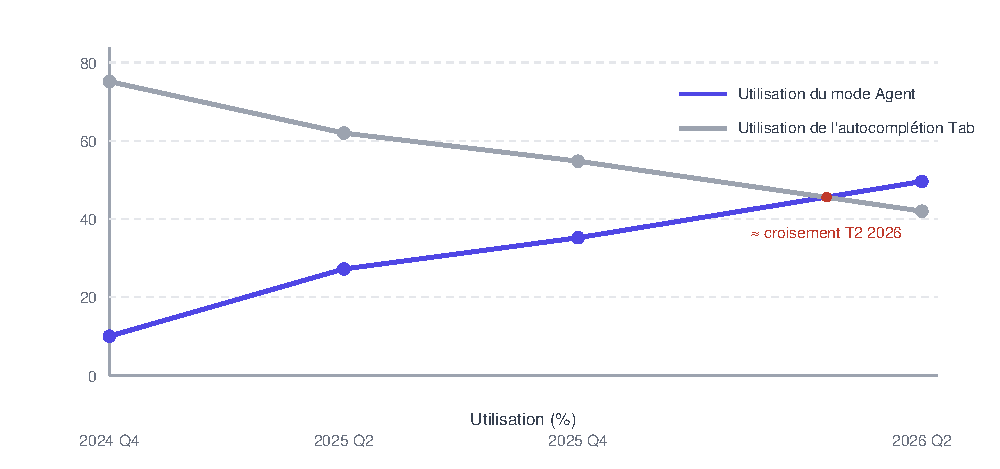
\includegraphics[width=0.92\linewidth]{figures/fig-di-san-shi-qi-zhang-1}
\\[2pt]\small Figure 1 : évolution de l'utilisation des modes d'interaction en programmation IA (estimation à partir d'études sectorielles ; au T2 2026, le mode Agent dépasse la complétion Tab)
\end{center}

Soyons lucides : l'évolution des outils et des modèles n'est que la surface. Que vous utilisiez Cursor ou Claude Code, GPT-5 ou Claude 4.5, les praticiens qui réussissent suivent la même méthodologie de fond. C'est ce que ce guide vous enseigne.

\booksection{III. Le grand basculement : de Coder à Conductor}

La formation traditionnelle fait de vous un Coder : comprendre la syntaxe, mémoriser les API, déboguer. À l'ère de l'IA, ce rôle se redéfinit. Vous n'écrirez plus chaque ligne, mais vous deviendrez un « chef d'orchestre » (Conductor) : définir le terrain, fixer les règles, répartir les tâches, valider les résultats.

Le cœur du changement n'est pas « savez-vous coder », mais « savez-vous clairement ce qu'il faut faire ». Un bon chef d'orchestre n'est pas forcément le meilleur soldat, mais il maîtrise l'objectif, le terrain et le déploiement. De même, un bon praticien IA n'a pas besoin de maîtriser chaque syntaxe, mais il doit maîtriser les objectifs du projet, ses contraintes d'architecture et ses standards de qualité.

Ce tableau mérite deux lectures — il résume tout le changement de rôle :

\begin{center}
\begin{tabularx}{\linewidth}{|X|X|X|}
\hline
\textbf{Dimension} & \textbf{Coder traditionnel} & \textbf{Conductor (chef d'orchestre IA)} \tabularnewline
\hline
Compétences clés & Mémorisation de la syntaxe, appels d'API, débogage & Définition des besoins, gestion du contexte, jugement d'acceptation \tabularnewline
Mode de travail & Écrire le code ligne par ligne & Décrire l'intention, examiner la production \tabularnewline
Contrôle qualité & On connaît son propre code & Vérifier la production de l'IA par tests et relecture \tabularnewline
Exigences de savoir & Maîtrise approfondie d'un langage/cadre & Vue large de la technique, compréhension profonde du métier \tabularnewline
Goulot d'étranglement & Vitesse de frappe et syntaxe & Clarté de la pensée et capacité d'expression \tabularnewline
Sources d'erreur & Erreurs de syntaxe, oublis de logique & Besoins flous, contexte insuffisant \tabularnewline
\hline
\end{tabularx}
\end{center}

\begin{center}\small\color{gray}Comparaison des dimensions Coder traditionnel vs Conductor IA\end{center}

Cela ne veut pas dire que le savoir technique est inutile. Bien au contraire : savoir lire le code de l'IA permet de le revoir et de le corriger ; comprendre structures de données et algorithmes permet de juger la pertinence de ses solutions. Le savoir fixe votre « plafond de commandement » — mais son rôle passe de l'outil d'exécution au fondement du jugement.

\booksection{IV. Pourquoi la méthodologie prime sur les outils}

Les outils évoluent tous les trois mois, la méthodologie met trois ans à évoluer. Apprendre à manipuler un outil peut devenir obsolète en trois mois ; maîtriser une façon de penser reste valable trois ans plus tard.

Beaucoup commencent par demander « quel est le meilleur outil ? » ou « quel est le modèle le plus puissant ? ». Ces questions ne sont pas inutiles, mais mal hiérarchisées. Le paysage d'août 2026 n'a plus rien à voir avec celui d'août 2025 — Trae, Qoder montent et descendent, Cursor passe d'extension à IDE indépendant puis à Cursor 3, Claude Code devient le choix dominant en terminal. Mais derrière ces bouleversements, les principes des praticiens qui réussissent n'ont presque pas changé.

C'est pourquoi ce livre ne gaspille pas ses pages à détailler un outil — ces contenus seraient périmés une fois écrits. Toute son énergie va à une méthodologie éprouvée : penser les besoins, communiquer avec l'IA, vérifier les livrables, itérer sans cesse. Avec cette méthodologie, vous maîtrisez n'importe quel outil ; en n'apprenant qu'un outil, vous repartez de zéro à chaque changement.

\begin{tcbinfo}{Mot rassurant pour les débutants}
Si vous débutez, ne vous laissez pas intimider par le mot « méthodologie ». Ce n'est pas une philosophie abstraite, mais un manuel de « comment penser face à un problème ». Comme en cuisine : suivre une recette, c'est l'outil ; comprendre pourquoi l'assaisonnement et le feu sont ainsi réglés, c'est la méthodologie. Ce livre part des concepts les plus simples, avec des exemples concrets pour chaque principe, afin que vous compreniez non seulement le « quoi », mais aussi le « comment ».

\end{tcbinfo}

\begin{tcbpractice}{À vous de jouer : prenez une « photo de rôle »}
Sur une feuille, répondez : (1) Comment utilisez-vous aujourd'hui l'IA pour coder (si vous l'avez déjà fait) ? (2) Vous ressemblez plutôt au « Coder » ou au « Conductor » du tableau ? (3) Comment aimeriez-vous décrire votre façon de travailler dans trois mois ? Glissez la feuille dans le livre et relisez-la après le chapitre 47 — le changement est plus rapide qu'on ne le croit.

\end{tcbpractice}

\begin{tcbsummary}{Résumé du chapitre}
\begin{itemize}
  \item En 2025, Karpathy a nommé « Vibe Coding » la révolution : coder par intention en langage naturel plutôt que ligne par ligne
  \item En 2026, l'Agentic Engineering : objectif fixé, délégation, l'IA planifie et exécute, l'humain valide
  \item Le mode Agent de Cursor 3 dépasse la complétion Tab ; Claude Code atteint 2,5 milliards de dollars de revenu annualisé
  \item Votre nouveau rôle : Conductor — définir le terrain, fixer les règles, répartir les tâches, valider
  \item Les outils changent tous les trois mois, la méthodologie tous les trois ans — apprenez la méthodologie, pas la manipulation
\end{itemize}

\end{tcbsummary}
